
\section{Question 2}
\label{part2}
\begin{itemize} 
\item Using the pages from Q1 (A4), download all TimeMaps (including TimeMaps with 404 responses, i.e. empty or null TimeMaps) 
\begin{itemize}
\item Upload all the TimeMaps to github
\end{itemize}

\item Build a CDF for \# of mementos for each original URI (i.e., x-axis = \# of mementos, y-axis = \% of links)
\item See: \url {http://timetravel.mementoweb.org/guide/api/} 

\end{itemize}
\subsection{Solution}
\begin{itemize}
 \item I used `timelapse'\cite{timelapse} library to retrieve TimeMaps of each of the URIs.
 \item `timelapse'\cite{timelapse} library extracts memento created date along with memento.
 \item Out of 9,800 URIs, TimeMaps are retrieved for 8200 which includes empty files.
 \item I ran multiple instances to retrieve TimeMaps as aggregator was taking time.
 \item Few times retrieval stopped because of request time out error. I waited for a few minutes before running it again.
 \item I have uploaded TimeMaps of each of the URIs to Github.
\end{itemize}

\lstinputlisting[language=Python,breaklines = true,frame=single,caption={Python program to retrieve TimeMap of each of the URIs}, label=lst:q1-1,captionpos=b,numbers=left,showspaces=false,showstringspaces=false,basicstyle=\footnotesize]{getmaps.py}

\begin{figure}[ht]
	\begin{center}
		 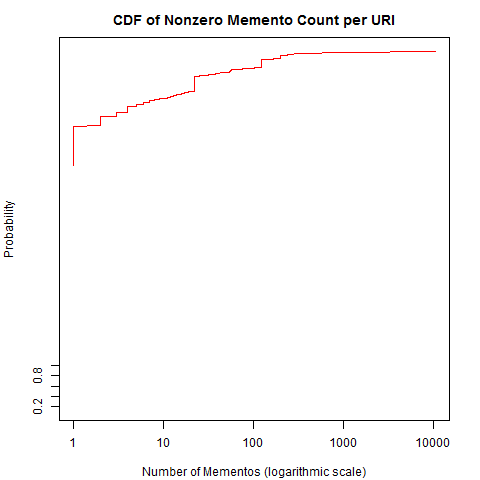
\includegraphics[scale=0.60]{mementocounts.png}
		  \caption{CDF of Number of Memento count per URI}
	 \end{center}
\end{figure}
\newpage
